\documentclass[11pt]{article}
\usepackage{geometry}           
\geometry{letterpaper}                   

\usepackage{graphicx}
\usepackage{amssymb}
\usepackage{epstopdf}
\usepackage{natbib}
\usepackage{amssymb, amsmath}
\usepackage{listings}
\usepackage{inconsolata}
\usepackage{xcolor}
\usepackage[nottoc,numbib]{tocbibind}
\usepackage{float}

\definecolor{codeRed}{RGB}{231,76,60}
\definecolor{codeBlue}{RGB}{52,152,219}
\definecolor{codePurple}{RGB}{155,89,182}
\definecolor{codeDarkBlue}{RGB}{52,73,94}

\lstdefinelanguage{JavaScript}{
  keywords={typeof, new, catch, function, null, catch, switch, if, in, while, do, else, case, break, for, return, continue},
  keywordstyle=\color{codeBlue}\bfseries,
  ndkeywords={class, export, boolean, throw, implements, import, this, var, let, const, int, double, char, true, false},
  ndkeywordstyle=\color{codePurple}\bfseries,
  identifierstyle=\color{codeBlue},
  sensitive=false,
  comment=[l]{//},
  morecomment=[s]{/*}{*/},
  commentstyle=\color{gray}\ttfamily,
  stringstyle=\color{codeRed}\ttfamily,
  morestring=[b]',
  morestring=[b]"
}

\lstset{
   language=JavaScript,
   backgroundcolor=\color{white},
   extendedchars=true,
   basicstyle=\footnotesize\ttfamily,
   showstringspaces=false,
   showspaces=false,
   numbers=left,
   numberstyle=\footnotesize,
   numbersep=9pt,
   tabsize=2,
   breaklines=true,
   showtabs=false,
   captionpos=b
}

\DeclareGraphicsRule{.tif}{png}{.png}{`convert #1 `dirname #1`/`basename #1 .tif`.png}

\title{Burning Man}
\author{Nico Hauser, Andri Horat, Elias Schmid, Jonas Spieler}
\date{date}

\begin{document}



\thispagestyle{empty}

\begin{center}
\includegraphics[width=5cm]{ETHlogo.eps}

\bigskip


\bigskip


\bigskip


\LARGE{ Burning Man:\\ }
\LARGE{ Simulating the behaviour of people in the event of fire\\}

\bigskip

\bigskip

\small{Project Report}\\

\bigskip

\bigskip

\bigskip

\bigskip


% \begin{tabular}{|c|}
% \hline
% \\
% \textbf{\LARGE{Burning Man}}\\
% \\
% \hline
% \end{tabular}
\bigskip

\bigskip

\bigskip

\LARGE{Nico Hauser, Andri Horat, Elias Schmid, Jonas Spieler}



\bigskip

\bigskip

\bigskip

\bigskip

\bigskip

\bigskip

\bigskip

\bigskip

Zurich\\
May 2008\\

\end{center}



\newpage

%%%%%%%%%%%%%%%%%%%%%%%%%%%%%%%%%%%%%%%%%%%%%%%%%

\newpage
\section*{Agreement for free-download}
\bigskip


\bigskip


\large We hereby agree to make our source code for this project freely available for download from the web pages of the SOMS chair. Furthermore, we assure that all source code is written by ourselves and is not violating any copyright restrictions.

\begin{center}

\bigskip


\bigskip


\begin{tabular}{@{}p{3.3cm}@{}p{6cm}@{}@{}p{6cm}@{}}
\begin{minipage}{3cm}

\end{minipage}
&
\begin{minipage}{6cm}
\vspace{2mm} \large Nico Hauser
 \vspace{\baselineskip}

\end{minipage}
&
\begin{minipage}{6cm}

\large Andri Horat

\end{minipage}
\\
\\
\\
\\
\\
\begin{minipage}{3cm}

\end{minipage}
&
\begin{minipage}{6cm}
\vspace{2mm} \large Elias Schmid

 \vspace{\baselineskip}

\end{minipage}
&
\begin{minipage}{6cm}

\large Jonas Spieler

\end{minipage}
\end{tabular}


\end{center}
\newpage

%%%%%%%%%%%%%%%%%%%%%%%%%%%%%%%%%%%%%%%



% IMPORTANT
% you MUST include the ETH declaration of originality here; it is available for download on the course website or at http://www.ethz.ch/faculty/exams/plagiarism/index_EN; it can be printed as pdf and should be filled out in handwriting


%%%%%%%%%% Table of content %%%%%%%%%%%%%%%%%

\tableofcontents

\newpage

%%%%%%%%%%%%%%%%%%%%%%%%%%%%%%%%%%%%%%%



\section{Abstract}

This paper describes a model for the behaviour of people in the event of an emergency situation and it's simulation. The model tries to incorporate the general repulsion of people standing too close, the formation of groups in panic situations, the placement of exit signs and many other factors such as different speeds. In order to make observations on the defined model, it is simulated using a physics engine written in javascript that makes it accessible from any place at any time and allows for reproducible and verifiable results. The paper defines a general parameterized model of the environment and the agents which, with the right choice of simulation parameters, may even allow for a safety evaluation of specific settings. Simulations using this model were able to verify results of other papers but also put them into perspective.

\section{Introduction and Motivations}

This paper was created during the course \textit{Agent-Based Modeling and Social System Simulation} held by Dr. Nino Antulov-Fantulin and Thomas Asikis at ETH Zurich. The goal was to create a project matching the title of the course meaning the modelling of a complex system where humans are the agents. A complex system is in contrast to complicated system not per se hard to implement but rather consists of many simple small parts that on themselves act based on simple rules. The fact that there are a lot of these so-called agents gives rise to behaviours of the whole system that are not always easy to predict or even understand even if the simple rules of a single agent are well-known. As computers keep getting faster and new technology is developed every day, simulations are a good way of understanding these complex systems by playing with the available parameters while looking for emerging patterns and then interpreting the implications for the real world.

\section{Description of the Model}

For readability this chapter is split as the definition of the environment is to some extent independent of the agent's model.

\subsection{Environment model}

Before agents can react to a fire an environment has to be created which in our case is a building. The environment model consists of walls, obstacles, doors and signs all of which are objects the agent interacts with. Walls are the most important part as they give the environment a shape and restricts the agent's movement. The same goes for obstacles, the reason why walls and obstacles are separated in our model is that the agent use a raytracing algorithm for finding a path and obstacles such as tables may prevent an agent from moving but do not interfere with their vision. Next are the doors and signs which also have similar roles. As it is the case in real life, safety signs guide an agent to the closest exit where agents are able to escape. Doors have the same effect on agents but represent something different as they're not a physical object but rather represent the agent's memory of where they entered a room. Both signs and doors are directional in our model as both, safety signs and doors, should only be used in one direction when escaping a building.

\subsection{Agent model}
For the agent model a so-called social force model is used. In short agents behave like particles in newtonian physics. Every agent has a mass, position and velocity and and the intentions and interactions of the agents are represented by forces. The agents are approximated as a circle in the physics engine where each agent has different intrinsic properties that are randomly generated using a normal distribution using a mean and a standard deviation. On one hand the circle radius of the agents is varied representing the different shoulder widths as it was done in \cite{Helbing}. In contrast to this paper, the desired velocity is chosen from a normal distribution as well as this seems more reasonable than all agents having exactly the same desired velocity. In addition we also randomly choose a reaction time that determines how fast an agent does get moving into a given direction.

After the generation of these random values, the agents are a sole product of their environment and their behaviour is based on a set of simple rules.

\begin{itemize}
    \item Wall repulsion
    
    To model human behaviour, agents should in general prefer to move away from walls as most humans prefer to have some space around them.

    \item Agent repulsion
    
    For the same reason people do not like to stand close to each other, especially not in emergency situations. The closer the distance is, the greater is the applied force on every pair of agents to move away from each other.

%    \item Agent attraction
%    
%    Even tough people do not like to stand close to each other, they still tend to form groups and do not like to act on their own. Thus the agents are instructed to move closer together as long as the distance between them is in the acceptable range.

    \item Target attraction
    
    Last but definitely not least the agents need a task. In the best case, they should try to reach one of the defined escape zones in order to safe themselves. In real life, safety signs guide people to these safe zones so the agents are instructed to always be on the lookout for visible signs guiding them to safety, so we do the same in our model and guide agents to the closest visible safety sign or door. In addition agents will remember what signs and doors they have already passed and won't go into the direction of the same sign or door twice. Should be signs and doors be placed in a strange order, this behaviour ensures that agents won't go into the wrong direction twice. An exception is made to this rule if an agent doesn't have a target anymore. Then they ''forget'' everything they visited before and start from scratch. This allows for some more complex behaviours such as an agent being pushed back into the room he just was in because of other agents rushing the hallway. If the memory wasn't cleared, the agent now wouldn't leave the room a second time which of course would be a real bad behaviour.
\end{itemize}

\section{Implementation}

The implementation of this model is done in javascript using a game library called phaser that already includes a physics engine and has means of drawing the result onto a \texttt{HTML} canvas meaning the whole simulation can easily be rendered on a webpage and doesn't require any setup.

\subsection{Environment construction}
As people are at least to some extent the product of their environment, it is very important that the simulations does not have a fixed environment in which all simulations take place. In fact it is one of the most important parameters when looking at the results, i.e. how many people survived a fire emergency. People in a totally enclosed room have no chance of escaping whereas agents sitting next to an escape zone will have no issues. To make the change of this parameter as accessible as possible, the implementation uses an open source format called \texttt{Tiled's map format} (TMX).

\begin{figure}[H]
	\centering
	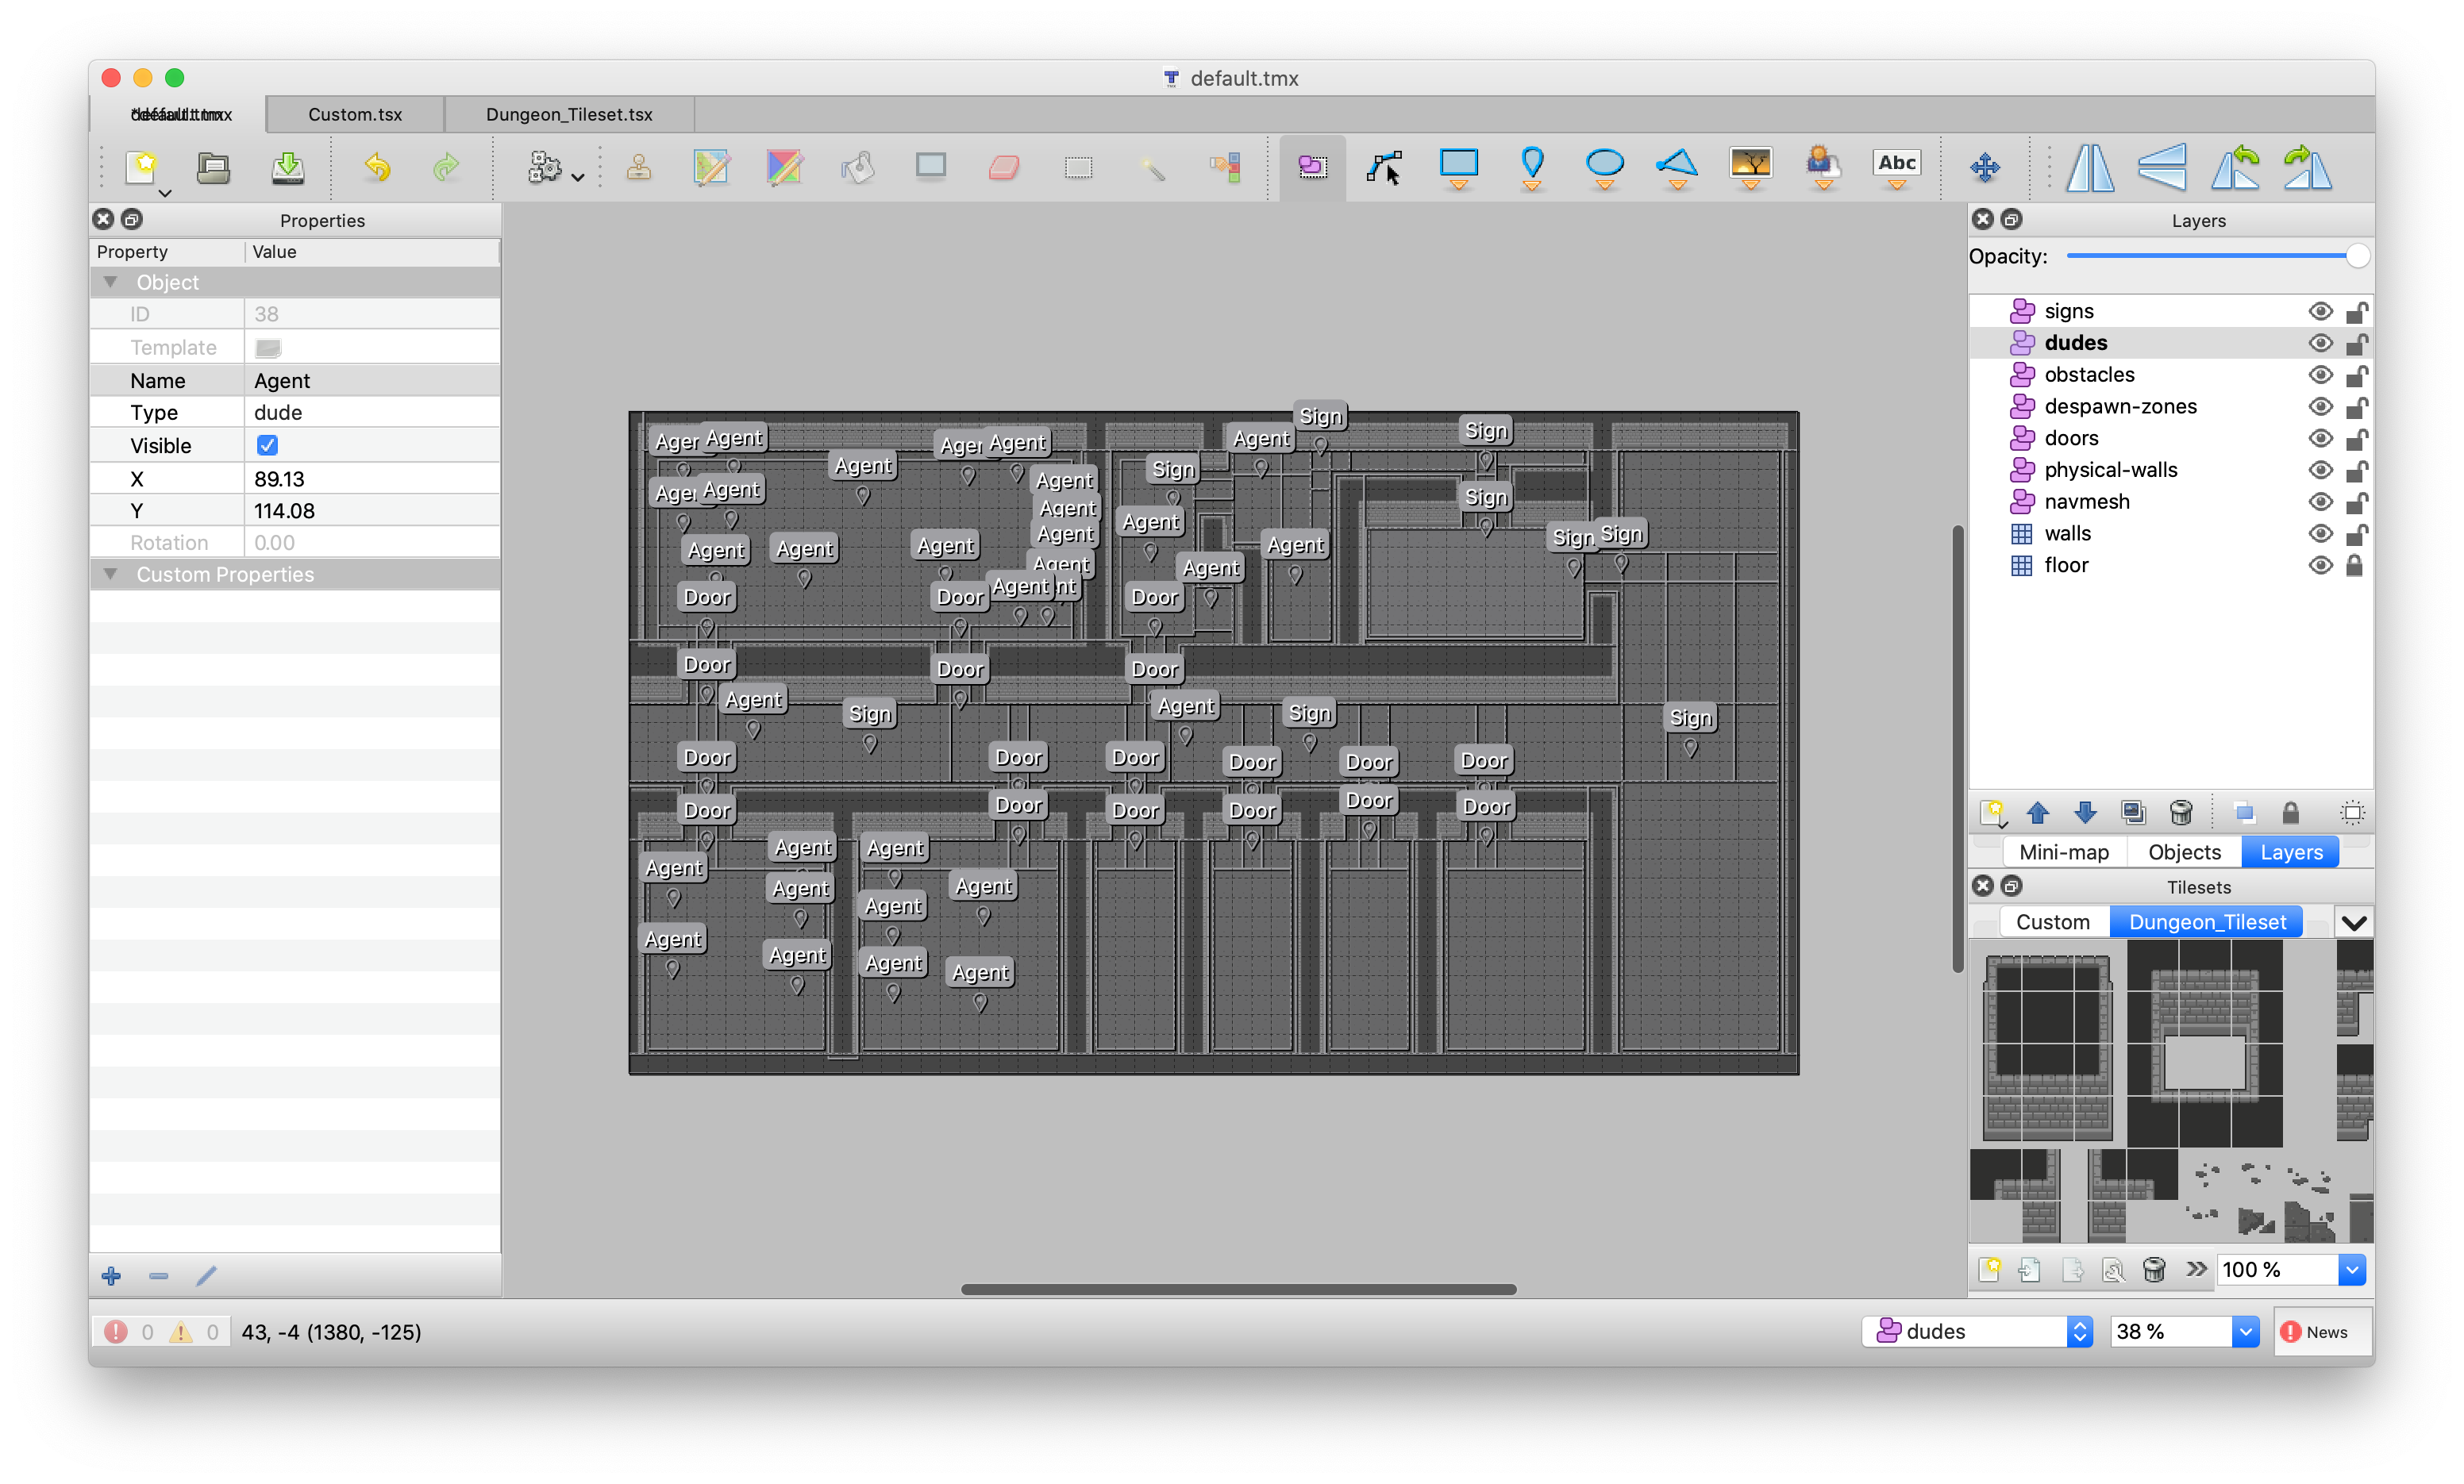
\includegraphics[width=1\linewidth]{assets/tiled-editor}\\
	The editing screen of Tiled
\end{figure}

Using this editor anyone with basic computer skills is able to adjust the given examples or of course define their own setting. This makes the model much more accessible and allows anyone to make their own tests using this model.

\subsection{Agent behaviour}

As phaser includes a physics engine we can make use of this by simulating the behaviour of the agents based on forces acting on them where the final movement is the vector addition of all these forces. Phaser has an \texttt{update} function that is called every time a new frame is calculated. which is perfectly suited for such a task. The different behavioural rules are implemented as follows

\begin{itemize}
    \item Wall repulsion
    
    -

    \item Agent repulsion
    
    Agent repulsion can be implemented rather easily: for every pair of agents a force
    
    \begin{align*}
    	f_r = c_1 \cdot e^{-\frac{d}{c_2}}
    \end{align*}
    
    where $c_1$ and $c_2$ are adjustable parameters but constant for the two agents and $d$ is the distance between the two agents. As the force is proportional to $e^{-d}$, the force is exponentially decreasing when linearly increasing the distance, i.e. exponentially increasing when linearly decreasing it. The initial values for $c_1$ and $c_2$ were empirically determined and are dependant on phaser's internal units.

%    \item Agent attraction
%    
%    The agent attraction force is, in contrast to the agent repulsion force, linearly dependant on the distance $d$
%    
%    \begin{align*}
%    	f_a = c_3 / d
%    \end{align*}
%    
%    but of course directed in the opposite direction of $f_r$. As $f_r$ is exponentially dependant on $d$ and $f_a$ just linearly there is a distance $d_0$ for which the two forces are in balance and the two agents will stay in place if no other force would act on them.

    \item Target attraction
    
    For checking what signs are visible, we iterate over all of them and use a technique called raytracing. This means we draw a line from the agent's position to the sign's position and check whether this line intersects any wall defined in the environment.
    
    \begin{minipage}{.1\textwidth}	
	\vfill\hfill
	\end{minipage}
    \begin{minipage}{.3\textwidth}
		\begin{figure}[H]
		\centering
		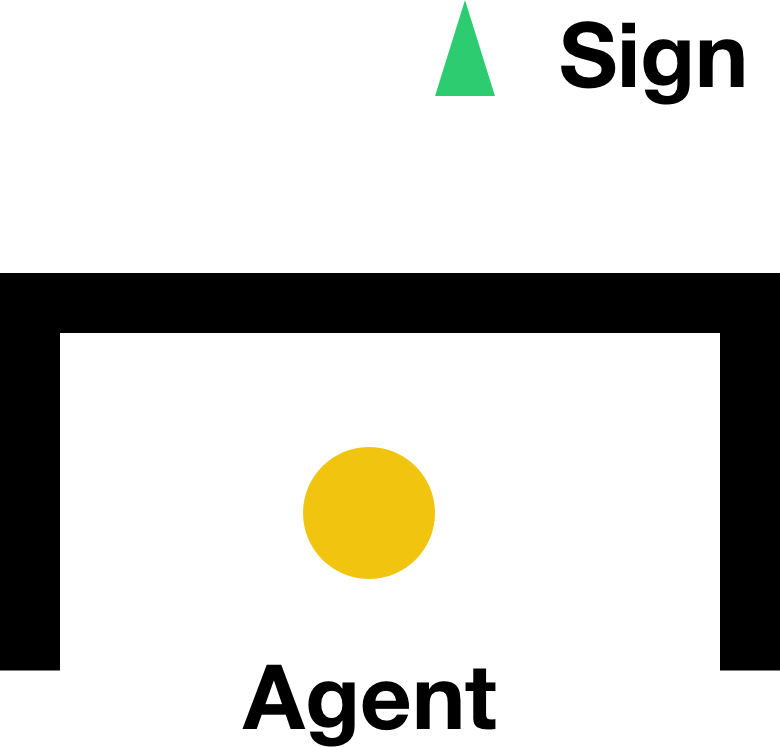
\includegraphics[width=1\linewidth]{assets/raytrace-blocked}\\
		An agent's vision blocked by a wall
	\end{figure}
	\end{minipage}
	\begin{minipage}{.2\textwidth}	
	\vfill\hfill
	\end{minipage}
	\begin{minipage}{.3\textwidth}
		\begin{figure}[H]
		\centering
		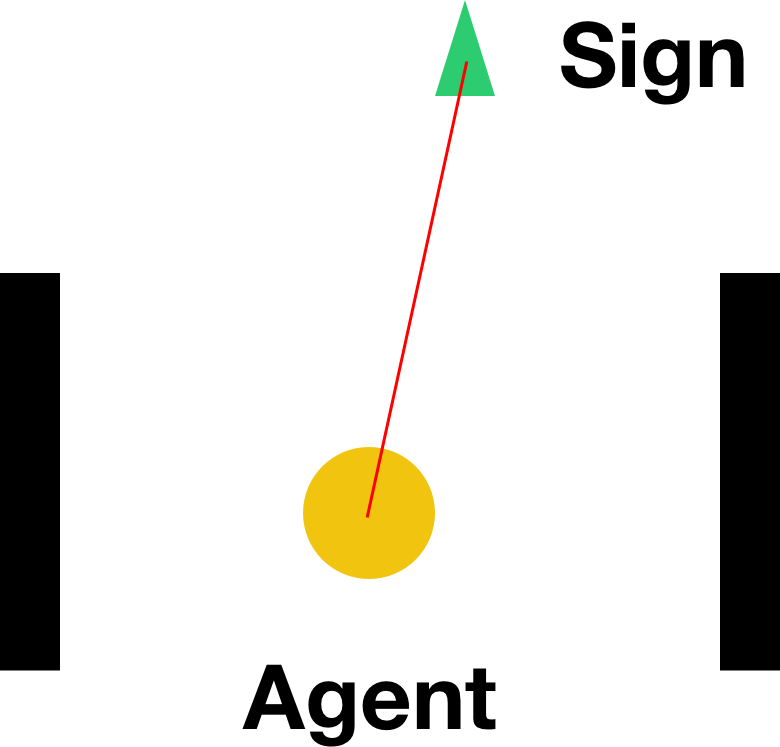
\includegraphics[width=1\linewidth]{assets/raytrace-visible}\\
		An agent's sight of a sign visualized by a red ''ray''
	\end{figure}
	\end{minipage}
    \\\\
	In the first figure above the agent is surrounded by walls meaning a line between the agent and the sign would intersect the front wall and thus in this case the agent wouldn't move towards the sign.
    
    If that's not the case, the sign is indeed visible and we can apply a force into the direction of the sign. This works fine until you introduce obstacles drawn in gray instead of black which stands for a wall. Obstacles collide with the agent as de walls, meaning the agent won't ''climb'' over it, the difference is that the agent can see ''through'' or over an obstacle. A good example for obstacles are tables.
	
	\begin{minipage}{.4\textwidth}
		\begin{figure}[H]
			\centering
			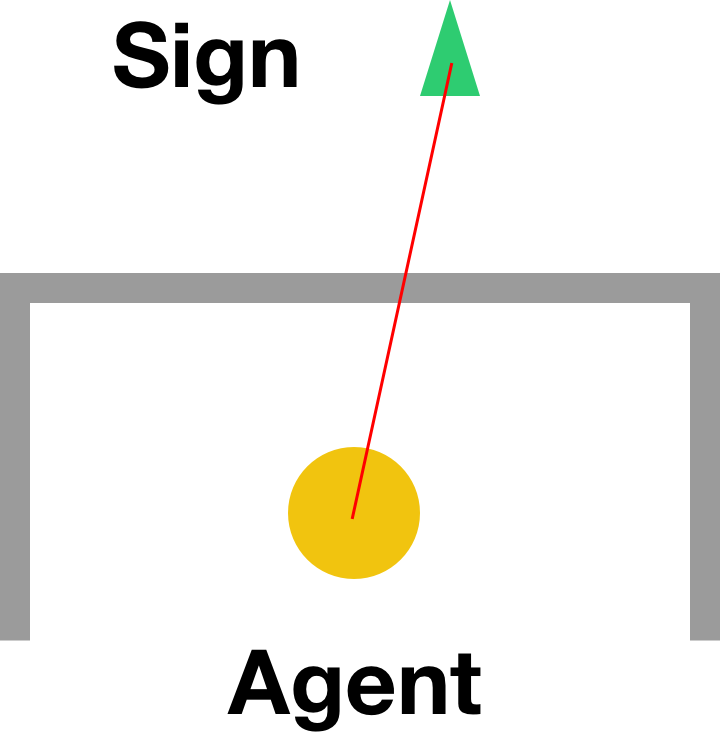
\includegraphics[width=.5\linewidth]{assets/without-navmesh}\\
			Agent stuck within obstacles
		\end{figure}
	\end{minipage}
	\begin{minipage}{.2\textwidth}	
	\vfill\hfill
	\end{minipage}
	\begin{minipage}{.4\textwidth}
		\begin{figure}[H]
			\centering
			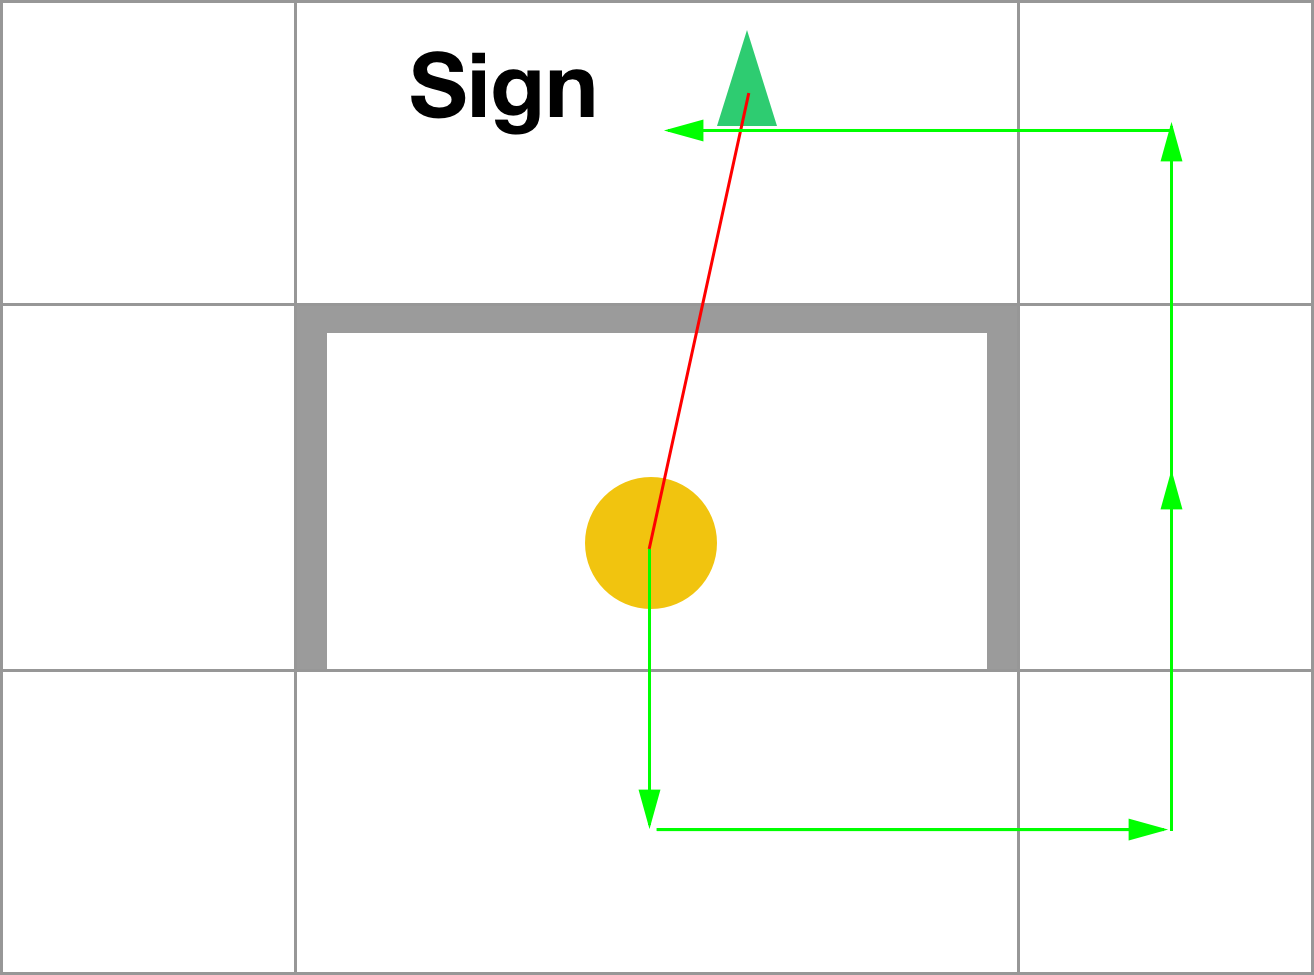
\includegraphics[width=1\linewidth]{assets/with-navmesh}\\
			Agent boxed in obstacles using pathfinding
		\end{figure}
	\end{minipage}
	
	Now the issue with directly applying a force to the agent into the direction of the ray becomes obvious, the agent will get stuck as it cannot move through the wall. To circumvent this issue, a so called pathfinding algorithm is used, once the agent sees a sign. Now the agent doesn't just move into the targets direction but rather finds a way to the target and this way is able to walk around obstacles. The pathfinding algorithm works by generating an ordered list of points that the agent can follow to get to the target position.
	
	As soon as we know the target of an agent, we can compute the velocity-correcting force, which tries to accelerate the current physical velocity $v_0$ of the agent to the desired velocity $v$. We compute the force by    
	\begin{align*}
	  f_t = m \cdot \frac{v_0-v}{\tau}
	\end{align*}
	where $m$ and $\tau$ are constants, that can be interpreted as the mass and the reaction time of an agent. In our simulation the $m$ is chooses based on the randomly chosen radius and $\tau$ is defined per agent and can be used directly.
    
\end{itemize}

\section{Simulation Results and Discussion}
To test our tool againt existing papers, we tried to replicate experiments of an existing article \cite{Helbing}. Our experiment 1 was described in \cite{Helbing}, whereas our experiment 2 was shown in the video that belongs to the article \cite{Helbing}.  


\subsection{Experiment 1}

For the first experiment we replicated the experiments from the paper \textit{Simulating dynamical features of escape panic} from Dirk Helbing, Illés Farkas and Tamás Vicsek in which the agents had to pass a bottleneck in an escape situation. The conclusion was there is an optimal velocity of about $1.5 m/s^-1$ at which all 200 agents left in the least amount of time.

\begin{minipage}{.4\textwidth}
		\begin{figure}[H]
			\centering
			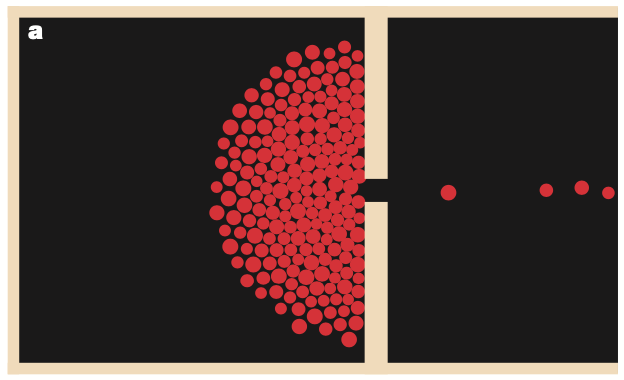
\includegraphics[width=1\linewidth]{assets/helbling-experiment-1}\\
			Setup from \cite{Helbing}
		\end{figure}
	\end{minipage}
	\begin{minipage}{.2\textwidth}	
	\vfill\hfill
	\end{minipage}
	\begin{minipage}{.4\textwidth}
		\begin{figure}[H]
			\centering
			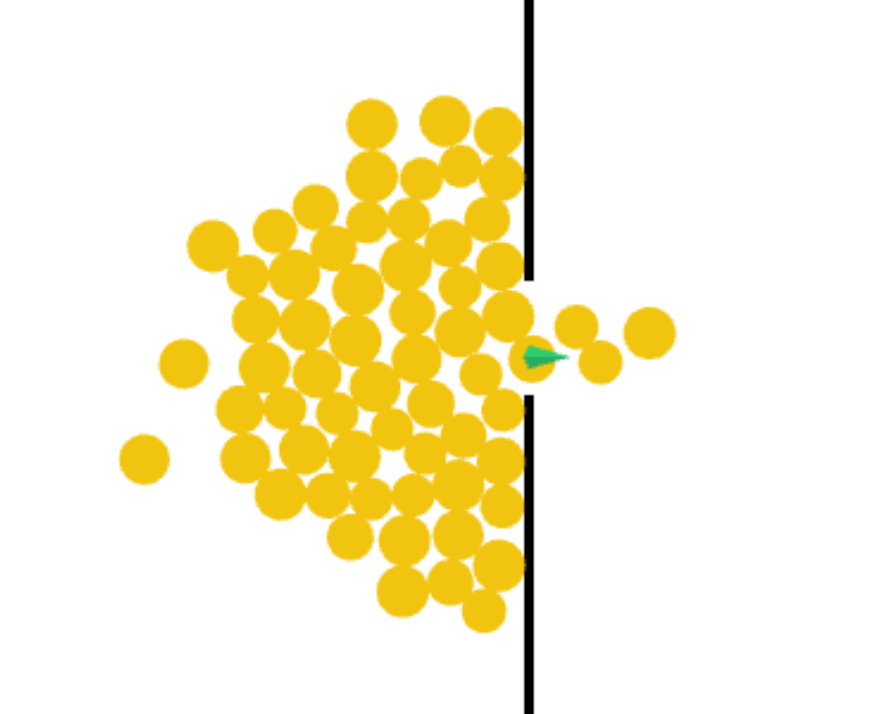
\includegraphics[width=.75\linewidth]{assets/experiment-1}\\
			This paper's setup
		\end{figure}
	\end{minipage}
	
We created a setup similar to that in \cite{Helbing} which is the right image above but in our model this simulation took different turns. When first trying it, some agents started glitching through the wall as the acting forces were extremely high. This is a known issue in physics engines as high forces imply high acceleration and velocity and we know from physics $s = s_0 + v\cdot t$. If physics engines directly calculate the new position in discrete time steps without verifying the path in between was clear, objects can glitch through walls without causing a collision. To circumvent this issue, we on one hand replaced the whole physics engine with a better one that verifies these cases but also reduced the number of agents. This lead to a new issue, not a physical one but one with the result: Suddenly we couldn't replicate the effect from the paper anymore, higher velocity almost always resulted in better escape times. When adjusting the friction between the agents this behaviour changed again and now most of the time all agents got indefinitely stuck in a situation similar to the one described in \cite{Helbing}. As we cannot create statistics where most of the time everyone gets stuck, it prevented us from having a similar nice statistic as Helbing, Farkas and Vicsek got. When comparing their results with ours, the differences are obvious. Most likely our model failed to replicate some important behaviour that was considered in \cite{Helbing} but it still seems interesting that he paper describes very exact what parameters were chosen for mass, acceleration time, desired velocity and so on but only mentions the friction very briefly, when saying ''if the friction parameter is large enough''\cite{Helbing}. Depending on how this sentence is interpreted, the results our model produced with a large friction parameter might be more similar than first thought and may also result from a different handling of the friction in the physics engines. It might be interesting to have a three-dimensional plot with the escape time over the desired velocity and the friction between the agents. Also the overall question remains whether a situation visible in the left image above can actually be used in respect to the escape time in real life as people would start to fall and others would start climbing and running over them. This wouldn't as drastically decrease the escape time for some but drastically for the ones getting hurt.

Even tough we could not directly verify alls results from \cite{Helbing}, the conclusion that higher escape velocities doesn't lead to faster escapes could be verified.

\begin{figure}[H]
	\centering
	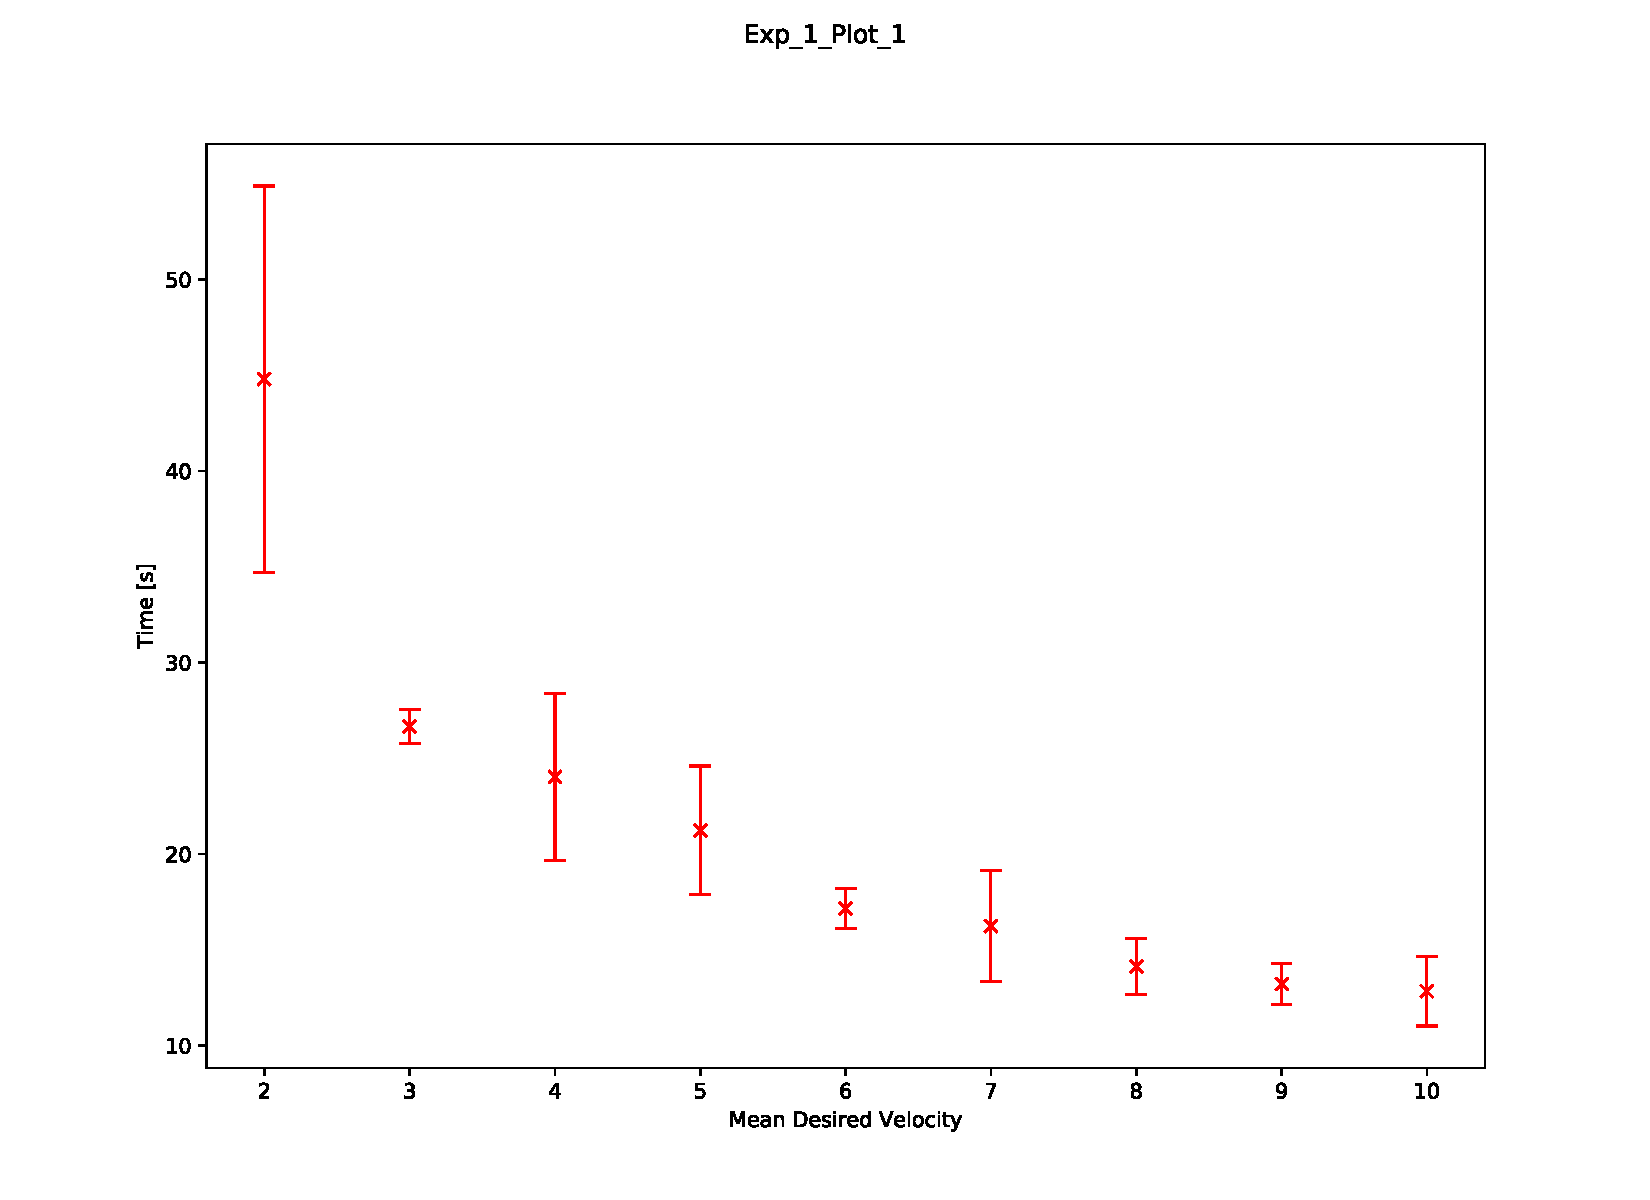
\includegraphics[width=.75\linewidth]{assets/Exp_1_Plot_1}\\
	Escape time over mean desired velocity
\end{figure}

As can be seen in the plot above, even tough the escape time continuously shrinks with increasing velocity, the difference keeps getting smaller and hits a minimum meaning further increasing the desired velocity won't further decrease the escape time. This plot is based on five runs per velocity on the described setting.

\subsection{Experiment 2}

\subsection{Experiment 3}

\subsection{Interpretation of the simulation result}
When running the simulation several times with a range of different parameters, we can observe some similar behaviour as it is already described in other articles.

\subsubsection{Clogging}
When running the simulation, one might notice that the agents competing for a door are closer together. This is due to the fact, that all agents are pushing towards the door, and hence pushing them together. It worsens the situation, as the friction between the agents increases, which slows down the escape.  
    
\subsubsection{Keeping the distance}
Interestingly, we can observe how agents are pushed back into rooms. Sometimes one could even witness how some agents use another path to avoid the crowd. This is actually what we would expect because of the mutual repulsion of the agents. 

\subsubsection{'Faster-is-Slower effect'}
There are already many published papers regarding the social-force-model. Of which many describe the 'Faster-is-Slower effect' \cite{Helbing, Wang}. The 'Faster-is-Slower effect' describes the phenomenon where the escape through an exit door is slower if the agents are pushing harder. When running our simulation on our default map, we did not observe this effect. The chances are, that this is due to the long corridor, where the agents make up time with a higher speed.

\subsection{Adapting the parameters for better results}

\subsection{Finding the model's limits}


\subsubsection{Evaluation of the building model}
\subsubsection{Evaluation of the agent model}
%The target attraction probably could have been modeled in a better way, instead of simply applying a force into the direction of the target, a real pathfinding algorithm could try to find the fastest way to the target that may involve walking around obstacles. In the current implementation agents fail to walk to the target if they are boxed in into the direction of the target.

\subsection{Evaluation of the simulation}

\section{Summary and Outlook}
- agents should only interact via forces if they can see each other (improve using raytracing)
- use empirical values for the parameters and constants
- use a more stable physics engine
- implement a random fluctuating force to prevent deadlocks

%\section{References}

%To add references, search the paper on https://www.researchgate.net/publication/12295370_Simulating_Dynamic_Features_of_Escape_Panic/citation/download
% and then copy the BibTeX Citation into the file refs.bib

\bibliographystyle{plain}
\bibliography{refs}

\end{document}  



 
